%!TEX root = ../thesis.tex
%*******************************************************************************
%*********************************** First Chapter *****************************
%*******************************************************************************
\graphicspath{{Chapter1/Figs/Vector/}{Chapter1/Figs/}}

%%%%%%%%%%%%%%%%%%%%%%%%%%%%%%%%%%%%%%%%%%%%%%%%%%%%%%%%%%%%%%%%%%%%%%%%%%%%%%%%
% Introduction
%%%%%%%%%%%%%%%%%%%%%%%%%%%%%%%%%%%%%%%%%%%%%%%%%%%%%%%%%%%%%%%%%%%%%%%%%%%%%%%%
% - Introduction to the introduction
% - Context
% - Restatement of the problem
% - Restatement of the response
% - Roadmap
%
\chapter{Introduction}
What was once an ordinary startup known as Uber, is now the most famous taxi dispatch company in the world \cite{Uber}. In the same year that Uber was founded, a similar startup in the Netherlands called taxiID was launched; an Amsterdam based company providing end-to-end cloud solutions for taxi companies. Hailing a taxi has rarely been performed by sticking out ones hand, hoping to catch the attention of a bypassing cab, ever since. Recently, taxiID has started developing a new brand called YourDriverApp (YDA). Opposed to the original taxiID brand, YDA is a lighter and newer version of the original solution, being more focussed on smaller taxi companies. Currently the functionalities that YDA provides depend on the legacy system. This chapter expands on this challenge and how it was translated into an assignment.

%%%%%%%%%%%%%%%%%%%%%%%%%%%%%%%%%%%%%%%%%%%%%%%%%%%%%%%%%%%%%%%%%%%%%%%%%%%%%%%%
% Context
%%%%%%%%%%%%%%%%%%%%%%%%%%%%%%%%%%%%%%%%%%%%%%%%%%%%%%%%%%%%%%%%%%%%%%%%%%%%%%%%
% - General
% - Clients
% - Structure
% - Cooperation
%
\section{Context}
% General
taxiID was founded as a startup that successfully introduced smartphone taxi booking in The Netherlands, and offers a wide range of IT solutions to serve the taxi market, including a passenger app, a driver app, and administrative panels. More specifically: an app for passengers to order a taxi, an app for drivers to receive their job assignments, and services  for all size businesses, offering convenient planning and dispatching without requiring local installations.
% Clients
Clients who make use of taxiID's services can be found anywhere in the world. This intoduces complicated challenges while developing applications that rely on clearly defined locations and infrastructures, often vastly differing between countries, if these countries have such a system to begin with.
% Structure
The taxiID development team is located in Medemblik, consisting of two mobile app developers (iOS and Android), two backend developers, a designer and two project managers.
% Cooperation
% Bridge

%%%%%%%%%%%%%%%%%%%%%%%%%%%%%%%%%%%%%%%%%%%%%%%%%%%%%%%%%%%%%%%%%%%%%%%%%%%%%%%%
% Problem Definition
%%%%%%%%%%%%%%%%%%%%%%%%%%%%%%%%%%%%%%%%%%%%%%%%%%%%%%%%%%%%%%%%%%%%%%%%%%%%%%%%
% -
%
\section{Problem Definition}
YDA requires its own pricing calculation functionality that is similar to the existing taxiID implementation. Similar in the sense that the system should return a formatted response that is identical to the existing system, where the content within the format may vary. But different in the way that it is architecturally set up, how the pricing rules are implemented, how ... \mynote{more reasons for problem definition}.

\begin{figure}[htbp!]
	\centering
	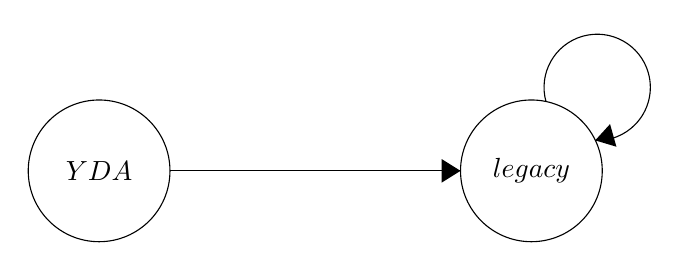
\begin{tikzpicture}[scale=0.3]
	\tikzstyle{every node}+=[inner sep=0pt]
	\draw [black] (23.7,-41.6) circle (3);
	\draw (23.7,-41.6) node {$YDA$};
	\draw [black] (42,-41.6) circle (3);
	\draw (42,-41.6) node {$legacy$};
	\draw [black] (26.7,-41.6) -- (39,-41.6);
	\fill [black] (39,-41.6) -- (38.2,-41.1) -- (38.2,-42.1);
	\draw [black] (42.62,-38.677) arc (195.76239:-92.23761:2.25);
	\fill [black] (44.7,-40.31) -- (45.6,-40.58) -- (45.33,-39.62);
	\end{tikzpicture}
	\label{fig:sub2}
	\caption[Dependencies]{YDA depending on legacy}
  \label{fig:dependencies}
\end{figure}


All functionalities within the current system align with the clients demands, but some features introduce difficulties, for example: region names are too vague for specific database queries. A system must be implemented in which group admins can define pricing rules based on user defined locations and time schedules, that can be used for calculating a passengers trip price, or show prices of different products based on the trip the passenger is about to make. In the current system, locations are uploaded by taxi company group admins as excel sheets with departure and destination zip codes in conjunction with prices. This process works in countries with an unambiguous, explicit, well-defined postal code infrastructure. Postal codes are matched in efficient database queries, leaving less room for improvement in terms of performance. Interpretability is an issue however. Sheets may contain thousands of rows, making it hard to interpret and maintain. On top of that, countries without such systems are not covered by the functionality. There are two more types of pricing rules that cover the rest of trip pricing cases.

%%%%%%%%%%%%%%%%%%%%%%%%%%%%%%%%%%%%%%%%%%%%%%%%%%%%%%%%%%%%%%%%%%%%%%%%%%%%%%%%
% Assignment
%%%%%%%%%%%%%%%%%%%%%%%%%%%%%%%%%%%%%%%%%%%%%%%%%%%%%%%%%%%%%%%%%%%%%%%%%%%%%%%%
% - Description
%
\section{Assignment}
The title of this thesis, as agreed upon by the Examination Committee, reads: \\
\textit{"A rule-based geospatial reasoning system for trip price calculations"}. \\

A system must be implemented that is capable of

A tier price system, that calculates fixed prices based cascading thresholds, and a dynamic pricing system that calculates prices per distance unit and minute. The term 'distance unit' is used on purpose, as distances are measured using different metrics in various countries. Pricing rules should be constrained by time frames, making rules available only for some hours a day, or only on christmas for example. Rules should be specifyable per product as different vehicle types have different prices, but are included in the same pricing rules. Discounts may be calculated with the trip price, and VAT should be displayed in the price breakdown. Some additional requirements to the system may be added in later phases, as Scrum is used to manage work iterations (this fact is covered later in this chapter). The system should be accessible to other systems, meaning that applications that currently rely on the old system should be able to migrate to the new system. As the old system shouldn't be used for new applications, as it was not designed for this use case. The system should have a single responsibility, and should be autonomous in that regard.

%%%%%%%%%%%%%%%%%%%%%%%%%%%%%%%%%%%%%%%%%%%%%%%%%%%%%%%%%%%%%%%%%%%%%%%%%%%%%%%%
% Research
%%%%%%%%%%%%%%%%%%%%%%%%%%%%%%%%%%%%%%%%%%%%%%%%%%%%%%%%%%%%%%%%%%%%%%%%%%%%%%%%
% - How to get the required knowledge
%
\section{Research}
% Hoe wordt dit onderzoek aangepakt?
% Designing research involves two separate sets of activities. The first involves determining everything you wish to achieve through the research project. This has to do with modelling the content of the research; we call this the con-ceptual design of a research project. The second set of activities concerns howto realise all this during the implementation stage of the project. This is called the technical research design.
Three main challenges that construct the assignment can be identified. Research must be done to attain the best possible way of mapping locations to pricing rules. What this means is that locations must be storable, comparable, and interpretable. The database must be able to store locations in an efficient manner, to which queries can be made as efficiently in order to find out whether a pricing rule applies to a given ride. For this to be the case, the stored locations must be comparable to the location of the passenger, or the destination. The user must be able to reason about his pricing rules, from which an understanding of his defined locations logically follows. But edge cases must be covered completely. For example, a rule in the current system dictates that a user traveling to Schiphol should receive a discount. But how would the system detect that this is the case? Or what if hotel guests receive discounts, but the neighbour shouldn't be allowed to use these discounts? Secondly, a system has to be developed that encapsulates the solution that is the result of the conducted research. It is helpful to extend the research of the problem to finding out how to incorporate the answers into a working system, where architecture has a major influence in the tools that are available. For example: if a solution to the main problem requires a database system capable of handling high quantities of geospatial queries, this requirement has to be satisfied in order to proceed in finding the final solution. Finally, a user interface has to be created that enables users to define the pricing rules. The complexity of the interface depends on how straight forward the price calculation system is put together. The user interface should also be available in multiple portals. The best way of making the systems capabilities available to the user through the UI in the portal, must be investigated. The UI must be built keeping the user in mind, simplifying complex rule management as much as possible.

\subsection{Questions}

From the description of the problem, one main important research question can be derived: \textit{How can a generic location-based price calculation system be implemented that could be used in every country?} \\

This question encapsulates the three important challenges that have to be dealt with before the project can successfully be implemented. In order to give a clear direction to the research, sub-questions are separated into three groups; location mapping, architecture and user interface.

\begin{enumerate}

	\item In what way can locations be represented to be universally interpretable?
	      \begin{enumerate}[label*=\arabic*.]
		      \item Which types of locations should be distinguished?
		      \item What are the main differences between postal systems used around the globe?
		      \item Can postal codes be abstracted to geospatial data while retaining the same usefulness in the system?
		      \item How can different types of locations be effectively stored in a database?
	      \end{enumerate}

	\item How could the price calculation system be integrated into the existing architecture?
	      \begin{enumerate}[label*=\arabic*.]
		      \item Which architectural patterns fit in with the exising architecture?
		      \item How will authentication be handled?
		      \item How is identity management handled?
	      \end{enumerate}

	\item How can a working system be realized while defining rules is as insightful as possible to the user?
	      \begin{enumerate}[label*=\arabic*.]
		      \item Which Database Management System (DBMS) is suited for this project?
		      \item Which views should exist, does a logical hierarchy exist among views?
		      \item How should locations be defined and managed by the user?
		      \item How should timeframes be handled in the interface?
	      \end{enumerate}

\end{enumerate}

The first group of questions is answered in the chapter \mynote{Add chapter name}. The second and third is answered in the chapter Proposed Approach. At that point, enough knowledge is available to implement a solution.

%%%%%%%%%%%%%%%%%%%%%%%%%%%%%%%%%%%%%%%%%%%%%%%%%%%%%%%%%%%%%%%%%%%%%%%%%%%%%%%%
% Process
%%%%%%%%%%%%%%%%%%%%%%%%%%%%%%%%%%%%%%%%%%%%%%%%%%%%%%%%%%%%%%%%%%%%%%%%%%%%%%%%
% - How to complete the final product
%
\section{Process}

A written working method is provided to the product owner, see Appendix \ref{appendix:pregame}, Pregame. The documents purpose is to clearly define the assignment and document the interpretation of the assignment definition so that miscommunications are found immediately. Requirements, scope and stakeholders of the project, as well as laying out the project timeline and estimated architecture based on use cases are clearly documented. Finally, a proposed solution is the result, which is agreed upon by the product owner before the backlog is created. Reading the document is recommended if more knowledge about the process and context of the assignment is desired.
